\section{Experimental Results}
\label{sec:experiment}

\begin{table}
\caption{Statistics of trajectory dataset}
\label{tab:data}
\centering\small
\begin{tabular}{lrrrrr} \hline
\textbf{Dataset} & \textbf{\#Photos} & \textbf{\#Visits} & \textbf{\#Traj.} & \textbf{\#Users} \\ \hline
Edinburgh & 82,060 & 33,944 & 5,028 & 1,454 \\
Glasgow & 29,019 & 11,434 & 2,227 & 601 \\
Melbourne & 94,142 & 23,995 & 5,106 & 1,000 \\
Osaka & 392,420 & 7,747 & 1,115 & 450 \\
Toronto & 157,505 & 39,419 & 6,057 & 1,395 \\
\hline
\end{tabular}
\end{table}


\begin{table}
\caption{Characteristics of different algorithms}
\label{tab:algsummary}
\centering\small
\setlength{\tabcolsep}{3pt} % tweak the space between columns
\begin{tabular}{l|*{5}{c}} \hline
                                  & Query    & POI      & Trans. & No sub- & Joint        \\ 
                                  &          &          &        & tours   &         \\ \hline
\textsc{Random}                   & $\times$ & $\times$ & $\times$   & $\times$     & $\times$ \\
\textsc{PersTour}\cite{ijcai15}   & $\times$ & $\surd$  & $\times$   & $\surd$      & $\times$ \\
\textsc{PersTour-L}               & $\times$ & $\surd$  & $\times$   & $\surd$      & $\times$ \\
\textsc{PoiPopularity}            & $\times$ & $\surd$  & $\times$   & $\times$     & $\times$ \\
\textsc{PoiRank}                  & $\surd$  & $\surd$  & $\times$   & $\times$     & $\times$ \\
\textsc{Markov}                   & $\times$ & $\surd$  & $\surd$    & $\times$     & $\times$ \\
\textsc{MarkovPath}               & $\times$ & $\surd$  & $\surd$    & $\surd$      & $\times$ \\
\textsc{Rank}+\textsc{Markov}     & $\surd$  & $\surd$  & $\surd$    & $\times$     & $\times$ \\
\textsc{Rank}+\textsc{MarkovPath} & $\surd$  & $\surd$  & $\surd$    & $\surd$      & $\times$ \\
\textsc{StructuredSVM}            & $\surd$  & $\surd$  & $\surd$    & $\times$     & $\surd$  \\ \hline
\end{tabular}
\end{table}


\begin{table*}
\caption{Performance comparison on four datasets in terms of trajectory $F_1$-score.
         For each dataset (i.e., a column), the best method is shown in bold, the second best is shown in italic.}
\label{tab:f1}
\centering
\begin{tabular}{l|ccccc} \hline
 & Edinburgh & Glasgow & Melbourne & Osaka & Toronto \\ \hline
\textsc{Random} & $0.570\pm0.139$ & $0.632\pm0.124$ & $0.558\pm0.149$ & $0.621\pm0.117$ & $0.621\pm0.128$ \\
\textsc{PersTour}\cite{ijcai15} & $0.656\pm0.223$ & $\mathbf{0.802\pm0.213}$ & $0.491\pm0.211$ & $0.702\pm0.230$ & $0.720\pm0.215$ \\
\textsc{PersTour-L} & $0.651\pm0.143$ & $0.660\pm0.102$ & $0.578\pm0.140$ & $0.691\pm0.138$ & $0.642\pm0.112$ \\
\textsc{PoiPopularity} & $\mathbf{0.701\pm0.160}$ & $0.745\pm0.166$ & $0.621\pm0.136$ & $0.661\pm0.128$ & $0.679\pm0.120$ \\
\textsc{PoiRank} & $\mathit{0.694\pm0.157}$ & $\mathit{0.777\pm0.171}$ & $\mathbf{0.626\pm0.137}$ & $0.679\pm0.112$ & $\mathbf{0.748\pm0.166}$ \\
\textsc{Markov} & $0.629\pm0.172$ & $0.714\pm0.168$ & $0.577\pm0.168$ & $0.679\pm0.162$ & $0.663\pm0.157$ \\
\textsc{MarkovPath} & $0.678\pm0.148$ & $0.735\pm0.170$ & $0.596\pm0.147$ & $0.706\pm0.154$ & $0.689\pm0.140$ \\
\textsc{Rank+Markov} & $0.642\pm0.171$ & $0.736\pm0.176$ & $0.598\pm0.169$ & $0.701\pm0.171$ & $0.689\pm0.170$ \\
\textsc{Rank+MarkovPath} & $0.684\pm0.151$ & $0.760\pm0.170$ & $\mathit{0.625\pm0.150}$ & $\mathbf{0.719\pm0.161}$ & $0.724\pm0.152$ \\
\textsc{StructuredSVM} & $0.659\pm0.186$ & $0.727\pm0.173$ & $0.597\pm0.171$ & $\mathit{0.715\pm0.170}$ & $\mathit{0.728\pm0.186}$ \\
\hline
\end{tabular}
\end{table*}


\begin{table*}
\caption{Performance comparison on four datasets in terms of pair-$F_1$.
         For each dataset (i.e., a column), the best method is shown in bold, the second best is shown in italic.}
\label{tab:pairf1}
\centering
\begin{tabular}{l|ccccc} \hline
 & Edinburgh & Glasgow & Melbourne & Osaka & Toronto \\ \hline
\textsc{Random} & $0.261\pm0.155$ & $0.320\pm0.169$ & $0.249\pm0.148$ & $0.305\pm0.145$ & $0.311\pm0.167$ \\
\textsc{PersTour}\cite{ijcai15} & $0.417\pm0.343$ & $\mathbf{0.646\pm0.366}$ & $0.225\pm0.274$ & $\mathit{0.491\pm0.377}$ & $0.503\pm0.353$ \\
\textsc{PersTour-L} & $0.359\pm0.207$ & $0.352\pm0.162$ & $0.268\pm0.143$ & $0.415\pm0.243$ & $0.331\pm0.159$ \\
\textsc{PoiPopularity} & $\mathit{0.436\pm0.259}$ & $0.509\pm0.299$ & $0.316\pm0.178$ & $0.363\pm0.195$ & $0.385\pm0.202$ \\
\textsc{PoiRank} & $0.424\pm0.249$ & $\mathit{0.565\pm0.312}$ & $0.322\pm0.186$ & $0.376\pm0.173$ & $\mathit{0.512\pm0.295}$ \\
\textsc{Markov} & $0.424\pm0.238$ & $0.488\pm0.283$ & $0.297\pm0.192$ & $0.449\pm0.262$ & $0.419\pm0.237$ \\
\textsc{MarkovPath} & $0.400\pm0.234$ & $0.492\pm0.298$ & $0.294\pm0.187$ & $0.445\pm0.268$ & $0.407\pm0.234$ \\
\textsc{Rank+Markov} & $0.434\pm0.251$ & $0.540\pm0.294$ & $\mathbf{0.357\pm0.210}$ & $0.483\pm0.277$ & $0.462\pm0.266$ \\
\textsc{Rank+MarkovPath} & $0.408\pm0.239$ & $0.532\pm0.304$ & $0.331\pm0.213$ & $0.470\pm0.284$ & $0.465\pm0.266$ \\
\textsc{StructuredSVM} & $\mathbf{0.440\pm0.267}$ & $0.529\pm0.283$ & $\mathit{0.352\pm0.213}$ & $\mathbf{0.508\pm0.292}$ & $\mathbf{0.520\pm0.311}$ \\
\hline
\end{tabular}
\end{table*}


\begin{figure*}[htbp]
	\centering
	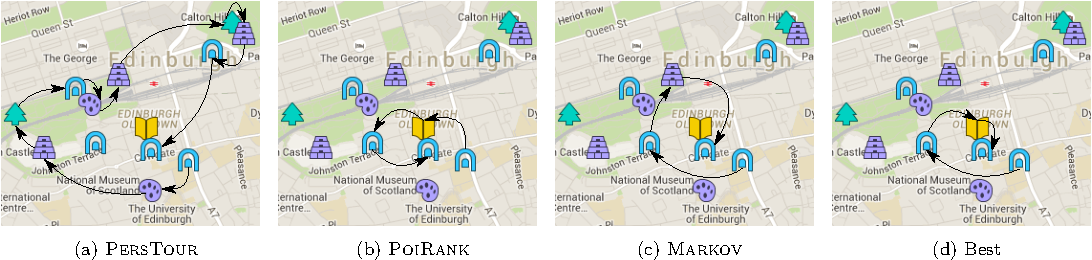
\includegraphics[width=\textwidth]{fig/example-tour.pdf}
	\caption{A figure illustrating results of different results from algorithm variants. 
}
	\label{fig:exampleresult}
\end{figure*}


\subsection{Dataset}
\label{sec:dataset}
We experiment on five trajectory datasets, four of them were provided by \cite{ijcai15}.
Trajectories in these datasets were extracted from Yahoo! Flickr Creative Commons 100M
(a.k.a. YFCC100M) dataset\cite{thomee2016yfcc100m} using metadata of photos and videos
such as geographical locations, timestamps, user identifications etc,
the details of building trajectories are covered in \cite{ht10} and \cite{ijcai15} and
we refer interested readers to these papers.
Statistics of the four trajectory datasets are described in table \ref{tab:data}.
%
The time that a user arrived a POI was approximated by the time the first photo taken by the user at that POI,
similarly, the time that a user leaved a POI was approximated by the time the last photo taken by the user at
that POI \cite{ht10, ijcai15}.


\subsection{Performance metric}
\label{sec:metric}

\cheng{Let's try this here. Still needs polishing.}

To evaluate the performance of different trajectory recommendation algorithms,
we employ the trajectory $F_1$-score\cite{ijcai15} to measure the POIs that are
correctly recommended. Let $\mathcal{T}$ be the trajectory that was visited in the real world,
and $\hat{\mathcal{T}}$ be the recommended trajectory,
$\mathcal{P}_{\mathcal{T}}$ be the set of POIs visited in $\mathcal{T}$,
and $\mathcal{P}_{\hat{\mathcal{T}}}$ be the set of POIs visited in $\hat{\mathcal{T}}$,
trajectory $F_1$-score was defined as
\begin{displaymath}
F_1= \frac{2 \times P_{\textsc{point}} \times R_{\textsc{point}}}
          {P_{\textsc{point}} + R_{\textsc{point}}}
\end{displaymath}
where
\begin{displaymath}
P_{\textsc{point}} = \frac{|\mathcal{P}_{\mathcal{T}} \cap \mathcal{P}_{\hat{\mathcal{T}}}|}
                          {|\hat{\mathcal{T}}|},
R_{\textsc{point}} = \frac{|\mathcal{P}_{\mathcal{T}} \cap \mathcal{P}_{\hat{\mathcal{T}}}|}
                          {|\mathcal{T}|}
\end{displaymath}

A perfect trajectory $F_1$-score (i.e., $F_1 = 1$) means the POIs in 
the recommended trajectory are exactly the same POIs as those in the ground truth, 
and $F_1 = 0$ means that unfortunately none of the POIs in the 
real trajectory was recommended.

In addition, to measure the quality of recommended visiting order of POIs,
we propose a new metric $\text{pair-}F_1$,
\begin{displaymath}
\text{pair-}F_1 = \frac{2 \times P_{\textsc{pair}} \times R_{\textsc{pair}}}
                       {P_{\textsc{pair}} + R_{\textsc{pair}}}
\end{displaymath}
where
\begin{displaymath}
P_{\textsc{pair}} = \frac{N_c} {|\hat{\mathcal{T}}|(|\hat{\mathcal{T}}|-1) / 2},
R_{\textsc{pair}} = \frac{N_c} {|\mathcal{T}|(|\mathcal{T}|-1) / 2}
\end{displaymath}
and $N_c$ is the number of POI pairs $(p_j, p_k)$ that satisfies the following
constraints\footnote{We define pair-$F_1=0$ if $N_c$ is $0$.}:
\begin{align*}
    (p_j \prec_{\mathcal{T}} p_k ~\land~ p_j \prec_{\hat{\mathcal{T}}} p_k) & ~\lor~
    (p_j \succ_{\mathcal{T}} p_k ~\land~ p_j \succ_{\hat{\mathcal{T}}} p_k) \\
    p_j \ne p_k, &~~ p_j, p_k \in \mathcal{P}_{\mathcal{T}} \cap \mathcal{P}_{\hat{\mathcal{T}}} \\
    j \ne k, &~~ 1 \le j, k \le |\mathcal{T}|
\end{align*}

A perfect pair-$F_1$, i.e., pair-$F_1 = 1$, means that both the POIs and their visiting order in the
recommended trajectory are exactly the same as these in the real trajectory,
and pair-$F_1 = 0$ means that none of the recommended POI pairs was actually visited in the real trajectory.


\subsection{Experimental Setup}
\label{sec:setup}
We use leave-one-out cross validation to evaluate different trajectory recommendation algorithms,
i.e., when evaluating a trajectory of a specific user, all other trajectories of this user as well as
all trajectories of other users were used to train the recommendation algorithms.

We conducted a comprehensive benchmark to compare the performance of different recommendation approaches.
In addition to the \textsc{PoiPopularity}, we also applied the \textsc{Random} baseline which naively chooses 
POIs uniformly at random (without replacement) from the set of POIs $\mathcal{P} \setminus \{p_s, p_e \}$ to visit.

Among the related approaches, \textsc{PersTour}\cite{ijcai15} is the most similar one, it formulated 
trajectory recommendation as an Orienteering Problem and use integer linear programming to maximise 
an objective, which composes both the POI popularity and user interest at the recommended POIs.
A user's interest on a specific category of POIs is modelled as the total ratios of his/her actual visit duration 
over the average visit duration at these POIs in general.
The recommended trajectory was also constrained by a time budget besides the origin and destination POIs.
To make further comparison, we replace the time budget in \textsc{PersTour} with the trajectory length and
denote this algorithm as \textsc{PersTour-L}.

Other recommendation approaches in this benchmark including \textsc{PoiRank} which utilises the ranking of POIs
described in section \ref{sec:ranksvm}, and \textsc{Markov} that recommending trajectories uses only transition 
probabilities between POIs, as described in section \ref{sec:transition}. Its variant \textsc{MarkovPath} that incorporates 
sub-tour elimination constraints described in section \ref{sec:walkpath} is also included.
Furthermore, \textsc{Rank+Markov} algorithm that leverage both POI ranking and transition probabilities as well as
its non-sub-tour variant \textsc{Rank+MarkovPath} that detailed in section \ref{sec:recommendation} are also 
benchmarked.

Lastly, we have the \textsc{StructuredSVM} that not only utilises POI ranking and transition probabilities but also 
jointly optimises their relative importance, as described in section \ref{sec:ssvm}.
The information that captured by these algorithms is summarised in table \ref{tab:algsummary},
and the associated parameters of these algorithms are detailed in the appendix.

% Parameters for IJCAI methods
The trade-off parameter for \textsc{PersTour} and \textsc{PersTour-L} was $0.5$, 
% Parameters for Heuristics
the trade-off value was used in \textsc{Rank+Markov} and \textsc{Rank+MarkovPath}.
% Parameters for rankSVM
The regularization parameter for rankSVM was $10$
% Parameters for SSVM
and $1$ for \textsc{StructuredSVM}.


\subsection{Results}
\label{sec:result}
% TODO: illustrate the recommendation results of figure \ref{fig:exampleresult} at the beginning of this section

% compare both F1 and pair F1 at the same time
The performance of ten algorithms on five trajectories datasets are shown in table \ref{tab:f1}
and table \ref{tab:pairf1} in terms of trajectory $F_1$-score and pair-$F_1$ respectively.
%
% 1. all vs Random 
% always better than Random, except PersTour on Melbourne which we'll illustrate later
It is obvious that algorithms captured a certain type of information in table \ref{tab:algsummary}
outperforms the \textsc{Random} baseline in terms of both metrics on all five datasets, 
except the performance of \textsc{PersTour}\cite{ijcai15} on Melbourne data which will be interpreted later.

% 2. PersTour vs. PersTour-L
% PersTour always better except on Melbourne which analysed later
\textsc{PersTour}\cite{ijcai15} always performs better than its variant \textsc{PersTour-L}, 
in particular on Glasgow and Toronto datasets, the advantage gap of \textsc{PersTour}
is significantly large in terms of both performance metrics,
%
% brief mention results of algorithms with and without utilising time budget constraint
which indicate the time budget constraint is more helpful than length constraint for recommending trajectories.
The exception on Melbourne dataset will again explained later.

% go to ranking based algorithms
Despite the utilisation of length constraint, algorithms based on ranking POIs yield very strong performance 
by exploring POI and query specific features.
%
% 3. PoiRank vs. PoiPopularity
% PoiRank yields nice improvement on four datasets, only slightly downgraded on Edinburgh
\textsc{PoiPopularity} baseline get pretty good performance despite its simplicity, 
and \textsc{PoiRank} yields nice improvements by leveraging more POI features and query specific features,
except slightly worse performance on Edinburgh dataset on which \textsc{PoiPopularity} is the best and 
second best performer in terms trajectory $F_1$-score and pair-$F_1$ respectively.

% go to transition based algorithms
On the other hand, Algorithm that leverage transition probabilities alone does not perform particularly well.
%
% 4. PoiRank vs. Markov: 
% in terms of F1, PoiRank always performs much better, except on Osaka where both yield comparable performance
In terms of trajectory $F_1$-score,
\textsc{Markov} can not outperform \textsc{PoiRank} except on Osaka dataset, 
on which the performance of both algorithms are comparable.

% in terms of pair F1, PoiRank is significantly better on Glasgow, Melbourne and Toronto, comparable on Edinburgh
In addition, \textsc{PoiRank} performs significantly better than \textsc{Markov} on three datasets, namely,
Glasgow, Melbourne and Toronto.
%
% at the first sight, it seems strange because Markov modelled the transitions and pair F1 measures the visiting order
% but actually pair F1 is affected heavily by the number of correctly predicted POIs, once the POIs are correctly predicted, it will yield 
% better pair F1, this is consistent with the observation that, on Osaka dataset, Markov and PoiRank yield comparable F1, 
% but Markov outperforms PoiRank significantly in terms of pair F1.
This result may seem strange at first sight because \textsc{Markov} modelled the transition pattern and it would leverage
this advantage to accomplish better performance in terms of pair-$F_1$ given the fact that this metric is measuring the quality
of visiting order.
However, pair-$F_1$ is actually affected heavily by the proportion of correctly recommended POIs in trajectory,
once the POIs are correctly predicted, a better pair-$F_1$ would be achieved, 
this supposition can be confirmed by the observation that, on Osaka dataset, \textsc{Markov} and \textsc{PoiRank} achieved
comparable performance in terms of trajectory $F_1$-score, which means the proportion of corrected recommended POIs is comparable,
\textsc{Markov} outperforms \textsc{PoiRank} significantly in terms of pair-$F_1$,
which suggest the transition information is helpful in some situations.

% 5. PoiRank vs. Markov vs. Rank+Markov
% in terms of both F1 and pair F1,
% when the advantage of PoiRank over Markov is large, Rank+Markov always brings improvements on Markov, but can't compete with PoiRank
% as the advantage gap of PoiRank over Markov shrinks, performance of Rank+Markov becomes closer to PoiRank,
% when the Markov is comparable or better than PoiRank, Rank+Markov outperforms both (Osaka)
% which is consistent with the assumption that transition helps when ranking didn't performs very well
In particular, when the advantage of \textsc{PoiRank} over \textsc{Markov} is large, 
i.e. Edinburgh, Glasgow, Melbourne and Toronto in table \ref{tab:f1} and Glasgow, Toronto in table \ref{tab:pairf1},
transition information is not very helpful as \textsc{Rank+Markov}, an algorithm that explores both POI ranking and transitions,
can not compete with \textsc{PoiRank} in both metrics, but nevertheless brings improvements to \textsc{Markov}.
However, as the performance of \textsc{Markov} approaches or surpasses that of \textsc{PoiRank}, 
i.e., Osaka in table \ref{tab:f1} and Edinburgh, Melbourne, Osaka in table \ref{tab:pairf1},
\textsc{Rank+Markov} outperforms both, this observation indicates that transition information can be very helpful when 
ranking does not performs well enough.

% 6. xxPath vs. xx:
% MarkovPath vs Markov: 
% in terms of F1, MarkovPath (Rank+MarkovPath) is always better than Markov (Rank+Markov),
% in terms of pair F1, MarkovPath (Rank+MarkovPath) yields comparable or worse performance than Markov.
% which indicates that sub-tour elimination helps POI prediction but worsen the visiting order.
Sub-tour has a non-ignorable effect when recommending trajectories.
From table \ref{tab:f1}, we can see both \textsc{Markov} and \textsc{Rank+Markov} can not compete with
their non-sub-tour counterparts, namely, \textsc{MarkovPath} and \textsc{Rank+MarkovPath}, 
in terms of trajectory $F_1$-score, which is not unexpected as sub-tours worsen the proportion of corrected
recommended POIs when length constraint is used.
On the contrary, they achieve better performance in terms of pair-$F_1$ which indicates sub-tours generally 
respect the visiting order between POIs.
 
% go to SSVM
The effect of sub-tours on trajectory recommendation can also be observed through the performance of \textsc{StructuredSVM},
%
% 7. SSVM vs Rank+Markov and Rank+MarkovPath:
% while SSVM using the same features as Rank+Markov and Rank+MarkovPath, and took advantage of its significantly larger number of parameters
% but SSVM permit sub-tours
% in terms of F1, 
% it either yield comparable performance with the better performer (Osaka/Toronto) or with the worse performer (Edinburgh/Glasgow/Melbourne) 
% which indicate how hurt sub-tours hurts POI recommendation.
% on the other hand, in terms of pair F1.
% it takes advantage of the transition patterns and yields comparable (Glasgow/Melbourne) or better performance than both of them 
although it uses the same features as \textsc{Rank+Markov} and \textsc{Rank+MarkovPath},
and can further take advantage of the significantly larger number of parameters,
when measured in terms of trajectory $F_1$-score, \textsc{StructuredSVM} can only yield comparable performance
with the best performer among the three at most.
On the other hand, \textsc{StructuredSVM} makes the best use of transition pattern which leads to comparable or
better performance, in terms of pair-$F_1$, than both of them all the time.
This observation is consistent with the effect of sub-tours observed above
as \textsc{StructuredSVM} do permit the existence of sub-tours in recommended trajectories.

% 8. PersTour on Melbourne:
% we observed that PersTour was outperformed by Random on Melbourne dataset in terms of both F1 and pair F1.
% it turns out on Melbourne dataset, the many of the ILPs which PersTour solve to get the recommendation result are very hard ILP instances
% in the leave-one-out evaluation, although we utilise a large scale computing cluster with modern hardware,
% there are 12\% of evaluations are failed due to ILP solver can't find a feasible solution in a $2$ hours
% furthermore, a lot recommendations are suboptimal solutions of the ILP due to the $2$ timeout settings.
% which leads to PersTour, which is always a strong performer on other datasets, performs inconsistently on Melbourne dataset.
Lastly, we observed that \textsc{PersTour}, a very good performer in general, is outperformed by \textsc{Random} baseline
on Melbourne dataset in terms of both trajectory $F_1$-score and pair-$F_1$.
It turns out that, on this very dataset, many of the integer linear programming (ILP) problems 
which \textsc{PersTour} need to solve to get the recommendation results are hard ILP instances.
In the leave-one-out evaluation, although we utilised a large scale computing cluster with modern hardware,
there are still $12\%$ of evaluations failed due to the ILP solver can not find a feasible solution in $2$ hours.
Furthermore, a lot of recommendations are produced from suboptimal solutions of the corresponding ILPs due to 
the $2$ hours timeout setting, these results lead to the generally strong performer \textsc{PerTour} performs 
inconsistently on Melbourne dataset.
